\documentclass[12pt, titlepage]{article}

\usepackage{fullpage}
\usepackage[round]{natbib}
\usepackage{multirow}
\usepackage{booktabs}
\usepackage{tabularx}
\usepackage{graphicx}
\usepackage{float}
\usepackage{hyperref}
\usepackage{ulem}
\usepackage[usenames, dvipsnames]{color}


\hypersetup{
    colorlinks,
    citecolor=black,
    filecolor=black,
    linkcolor=red,
    urlcolor=blue
}
\usepackage[round]{natbib}

\newcounter{acnum}
\newcommand{\actheacnum}{AC\theacnum}
\newcommand{\acref}[1]{AC\ref{#1}}

\newcounter{ucnum}
\newcommand{\uctheucnum}{UC\theucnum}
\newcommand{\uref}[1]{UC\ref{#1}}

\newcounter{mnum}
\newcommand{\mthemnum}{M\themnum}
\newcommand{\mref}[1]{M\ref{#1}}

\title{SE 3XA3: Software Requirements Specification\\ChessAce}

\author{Team 18, Team MIF
		\\ Jerry Ke, kex1
		\\ Harry Fu, fuh6
		\\ Morgan Cui, cuim2
}

\date{\today}

\input{../../Comments}

\begin{document}

\maketitle

\pagenumbering{roman}
\tableofcontents
\listoftables
\listoffigures

\begin{table}[bp]
\caption{\bf Revision History}
\color{red}
\begin{tabularx}{\textwidth}{p{3cm}p{2cm}X}
\toprule {\bf Date} & {\bf Version} & {\bf Notes}\\
\midrule
Nov 9th, 2018 & 1.0 & Starting create the Module Guide \\
Nov 30th, 2018 & 2.0 & Reversion 1\\
\bottomrule
\end{tabularx}
\end{table}


%\newpage

\pagenumbering{arabic}

\section{Introduction}

\subsection{Overview}
The purpose of this project is to re-implement the open source package ChessOOP which allows two players to play a chess game on one device offline.

\subsection{Design Principles}
Decomposing a system into modules is a commonly accepted approach to developing
software.  A module is a work assignment for a programmer or programming
team~\citep{ParnasEtAl1984}.  We advocate a decomposition
based on the principle of information hiding~\citep{Parnas1972a}.  This
principle supports design for change, because the ``secrets'' that each module
hides represents likely future changes.  Design for change is valuable in SC,
where modifications are frequent, especially during initial development as the
solution space is explored.  ~\citep{Bokahari2018}

Our design follows the rules layed out by \citet{ParnasEtAl1984}, as follows:
\begin{itemize}
\item System details that are likely to change independently should be the
  secrets of separate modules.
\item Each data structure is used in only one module.
\item Any other program that requires information stored in a module's data
  structures must obtain it by calling access programs belonging to that module.
\end{itemize}

\subsection{context}

After completing the first stage of the design, the Software Requirements
Specification (SRS), the Module Guide (MG) is developed~\citep{ParnasEtAl1984}. The MG
specifies the modular structure of the system and is intended to allow both
designers and maintainers to easily identify the parts of the software. The MG also documents how the system meets both functional and non-functional requirements that we were specified in the SRS. The
potential readers of this document are as follows:

\begin{itemize}
\item New project members: This document can be a guide for a new project member
  to easily understand the overall structure and quickly find the
  relevant modules they are searching for.
\item Maintainers: The hierarchical structure of the module guide improves the
  maintainers' understanding when they need to make changes to the system. It is
  important for a maintainer to update the relevant sections of the document
  after changes have been made.
\item Designers: Once the module guide has been written, it can be used to
  check for consistency, feasibility and flexibility. Designers can verify the
  system in various ways, such as consistency among modules, feasibility of the
  decomposition, and flexibility of the design.~\citep{Bokahari2018}

After the creation of the MG, the Module Interface Specification(MIS) is created. The MIS explains the semantics and syntax of exported functions (input, output and exceptions) for each module, essentially providing further detail on each module that is specified in the MG.~\citep{calce_fenster_tatasciore_2016}
\end{itemize}

The rest of the document is organized as follows. Section
\ref{SecChange} lists the anticipated and unlikely changes of the software
requirements. Section \ref{SecMH} summarizes the module decomposition that
was constructed according to the likely changes. Section \ref{SecConnection}
specifies the connections between the software requirements and the
modules. Section \ref{SecMD} gives a detailed description of the
modules. Section \ref{SecTM} includes two traceability matrices. One checks
the completeness of the design against the requirements provided in the SRS. The
other shows the relation between anticipated changes and the modules. Section
\ref{SecUse} describes the use relation between modules.



\section{Anticipated and Unlikely Changes} \label{SecChange}

This section lists possible changes to the system. According to the likeliness
of the change, the possible changes are classified into two
categories. Anticipated changes are listed in Section \ref{SecAchange}, and
unlikely changes are listed in Section \ref{SecUchange}.


\subsection{Anticipated Changes} \label{SecAchange}

Anticipated changes are the source of the information that is to be hidden
inside the modules. Ideally, changing one of the anticipated changes will only
require changing the one module that hides the associated decision. The approach
adapted here is called design for
change.~\citep{Bokahari2018}

\begin{description}
\item[\refstepcounter{acnum} \actheacnum \label{acHardware}:] The specific
  hardware on which the software is running.
\item[\refstepcounter{acnum} \actheacnum \label{acInput}:] The format of the
  initial input data.
\item[\refstepcounter{acnum} \actheacnum \label{acParams}:] The parameter of the input data.
\item[\refstepcounter{acnum} \actheacnum \label{acOutput}:] The format of the final output/display mechanisum.
\item[\refstepcounter{acnum} \actheacnum \label{acTime}:]  How long for each turn is determined from input data.
\item[\refstepcounter{acnum} \actheacnum \label{acPlayers}:] The players' name and color is determined using the input data.
\item[\refstepcounter{acnum} \actheacnum \label{acGUI}:] The graphical user interface element such as the chess board style and the pictures of each chess pieces.
\item[\refstepcounter{acnum} \actheacnum \label{acDefault}:] Default settings for input.
\end{description}


\subsection{Unlikely Changes} \label{SecUchange}

The module design should be as general as possible. However, a general system is
more complex. Sometimes this complexity is not necessary. Fixing some design
decisions at the system architecture stage can simplify the software design. If
these decision should later need to be changed, then many parts of the design
will potentially need to be modified. Hence, it is not intended that these
decisions will be changed.

\begin{description}
\item[\refstepcounter{ucnum} \uctheucnum \label{ucIO}:] Input/Output devices
  (Input: File and/or Keyboard, Output: File, Memory, and/or Screen).
\item[\refstepcounter{ucnum} \uctheucnum \label{ucInput}:] There will always be
  a source of input data external to the software.
\item[\refstepcounter{ucnum} \uctheucnum \label{ucRule}:] The basic rule of the chess game could not be changed(the basic algorithm of this program intended not to be changed). 
\item[\refstepcounter{ucnum} \uctheucnum \label{ucMovment}:] Basic movements for each pieces could not be changed.   
\item[\refstepcounter{ucnum} \uctheucnum \label{ucBoard}:]  The numbers of rows and columns of chess board could not be changed.
\item[\refstepcounter{ucnum} \uctheucnum \label{ucPosition}:]  The initial position of each pieces could not be changed.
\item[\refstepcounter{ucnum} \uctheucnum \label{ucPlayers}:]  The number of players could not be changed.
\end{description}



\section{Module Hierarchy} \label{SecMH}

This section provides an overview of the module design. Modules are summarized
in a hierarchy decomposed by secrets in Table \ref{TblMH}. The modules listed
below, which are leaves in the hierarchy tree, are the modules that will
actually be implemented.

\begin{description}

\item
\textcolor{red}{\sout{Hardware-Hiding Module}}
% [\refstepcounter{mnum} \mthemnum \label{mHH}:] Hardware-Hiding Module}}

\item [\refstepcounter{mnum} \mthemnum \label{mPAR}:] Parameter Module
\item [\refstepcounter{mnum} \mthemnum \label{mT}:] Time Module
\item [\refstepcounter{mnum} \mthemnum \label{mP}:] Player Module
\item [\refstepcounter{mnum} \mthemnum \label{mGUI}:] GUI display Module
\item [\refstepcounter{mnum} \mthemnum \label{mB}:] Board Module
\item [\refstepcounter{mnum} \mthemnum \label{mOUT}:] Output Module
\item [\refstepcounter{mnum} \mthemnum \label{mC}:] Cell Module
\item [\refstepcounter{mnum} \mthemnum \label{mPI}:] Pieces Module
\end{description}


\begin{table}[h!]
\centering
\begin{tabular}{p{0.3\textwidth} p{0.3\textwidth} p{0.3\textwidth}}
\toprule
\textbf{Level 1} & \textbf{Level 2} & \textbf{Level 3} \\
\midrule


\textcolor{red}{\sout{{Hardware-Hiding Module}}} \\
\midrule

\multirow{5}{0.3\textwidth}{Behaviour-Hiding Module}\\

& \multirow{1}{0.3\textwidth}{Input module}&{Parameter module}\\
& \multirow{2}{0.3\textwidth}{Default module}&{Time module}\\
& \multirow{2}{0.3\textwidth}{}&{Player module}\\\\
& {GUI display module}\\
& {Board module}\\
& {Output Module} \\
\midrule


\multirow{2}{0.3\textwidth}{Software Decision Module}\\
& Cell module\\
& Pieces module\\
\bottomrule

\end{tabular}
\caption{Module Hierarchy}
\label{TblMH}
\end{table}



\section{Connection Between Requirements and Design} \label{SecConnection}

The design of the system is intended to satisfy the requirements developed in
the SRS. In this stage, the system is decomposed into modules. The connection
between requirements and modules is listed in Table \ref{TblRT}.


The system was designed to satisfy the requirements. The Main class connects all components together and ensures the program can be executed. Performance, Operational and Environment requirements are satisfied through the Hardware-hiding Module as it serves as a virtual hardware used by the rest of the system and provides the interface between the hardware and the software. So, the system can use it to display outputs or to accept inputs. The GUI display Module shows all the operations using graphic interface which can satisfy Look and Feel, Usability and Humanity requirements. Maintainablity requirement is satisfied by Board Module and Cell Module. The Board Module stores and shares data needed by other modules by using cell module, while the Cell Module initializes position of each piece of the game. 


\section{Module Decomposition} \label{SecMD}

Modules are decomposed according to the principle of ``information hiding''
proposed by \citet{ParnasEtAl1984}. The Secrets field in a module
decomposition is a brief statement of the design decision hidden by the
module. The Services field specifies what the module will do
without documenting how to do it. For each module, a suggestion for the
implementing software is given under the Implemented By title. If the
entry is OS, this means that the module is provided by the operating
system or by standard programming language libraries.  Also indicate if the
module will be implemented specifically for the software.

Only the leaf modules in the hierarchy have to be implemented. If a dash (\emph{--}) is shown, this means that the module is not a leaf and will not have to be implemented. Whether or not this module is implemented depends on the programming language selected.\\

%%%%%%%%%%%%%%%%%%%%%%%%%%%%%%%%%%%%%%%%

\textcolor{red}{\sout{Hardware Hiding Modules}}

\begin{description}
\item \textcolor{red}{\sout{[Secrets:]The data structure and algorithm used to implement the virtual hardware.}}
\item \textcolor{red}{\sout{[Services:]Serves as a virtual hardware used by the rest of the
  system. This module provides the interface between the hardware and the
  software. So, the system can use it to display outputs or to accept inputs.}}
\item\textcolor{red}{\sout{[Implemented By:] OS}}
\end{description}
%%%%%%%%%%%%%%%%%%%%%%%%%%%%%%%%%%%%%%%%%%

\subsection{Behaviour-Hiding Module}
\begin{description}
\item[Secrets:]The contents of the required behaviours.
\item[Services:]Includes programs that provide externally visible behaviour of
  the system as specified in the software requirements specification (SRS)
  documents. This module serves as a communication layer between the
  hardware-hiding module and the software decision module. The programs in this
  module will need to change if there are changes in the SRS.
\item[Implemented By:] --
\end{description}


\subsubsection{Input Module}
\begin{description}
\item[Secrets:]The inputs of data.
\item[Services:]Converts the input data into the data structure used by the input module.
\item[Implemented By:] --
\end{description}

\begin{itemize}
\item{Parameter Module (\mref{mPAR})}
\begin{description}
\item[Secrets:]The parameters of the input data.
\item[Services:]Converts the input parameters data into the data structure.
\item[Implemented By:] Java Libraries
\end{description}
\end{itemize}


\subsubsection{Default Module}
\begin{description}
\item[Secrets:]The default setting of the game.
\item[Services:]Provides users the default setting to the game used by the default module.
\item[Implemented By:]--
\end{description}

\begin{itemize}
\item{Time Module (\mref{mT})}
\begin{description}
\item[Secrets:] The time setting of the game. 
\item[Services:] Allows users to set the timing before the game starting by using parameter module. 
\item[Implemented By:] Java Libraries
\end{description}
\end{itemize}

\begin{itemize}
\item{Player Module (\mref{mP})}
\begin{description}
\item[Secrets:]The player setting of the game. 
\item[Services:] Allows users to set players before the game starting by using parameter module.
\item[Implemented By:] Java Libraries
\end{description}
\end{itemize}


\subsubsection{GUI display Module(\mref{mGUI})}
\begin{description}
\item[Secrets:] All the operations.
\item[Services:] Shows all the operations using graphic interface by using pieces module.
\item[Implemented By:] Java Libraries
\end{description}


\subsubsection{Board Module (\mref{mB})}
\begin{description}
\item[Secrets:]Data
\item[Services:]Stores and shares data needed by other modules by using cell module.
\item[Implemented By:] Java Libraries
\end{description}


\subsubsection{Output Module (\mref{mOUT})}
\begin{description}
\item[Secrets:] End game and checkmate.
\item[Services:]Provides the result of the game by using board module.
\item[Implemented By:] Java Libraries
\end{description}



\subsection{Software Decision Module}

\begin{description}
\item[Secrets:] The design decision based on mathematical theorems, physical
  facts, or programming considerations. The secrets of this module are
  not described in the SRS.
\item[Services:] Includes data structure and algorithms used in the system that
  do not provide direct interaction with the user. 
  % Changes in these modules are more likely to be motivated by a desire to
  % improve performance than by externally imposed changes.
\item[Implemented By:] N/A
\end{description}

\subsubsection{Cell Module (\mref{mC})}

\begin{description}
\item[Secrets:] Position of pieces.
\item[Services:]Initializes position of each piece of the game by using pieces module.
\item[Implemented By:] Java Libraries
\end{description}

\subsubsection{Pieces Module (\mref{mPI})}

\begin{description}
\item[Secrets:] Possible movement of each piece.
\item[Services:] Highlights possible movenment each turn by using parameter module.
\item[Implemented By:] Java Libraries
\end{description}



\section{Traceability Matrix} \label{SecTM}

This section shows two traceability matrices: between the modules and the
requirements and between the modules and the anticipated changes.

% the table should use mref, the requirements should be named, use something
% like fref
\begin{table}[H]
\centering
\begin{tabular}{p{0.2\textwidth} p{0.6\textwidth}}
\toprule
\textbf{Req.} & \textbf{Modules}\\
\midrule
FR1 & \mref{mPAR}, \mref{mPI}\\
FR2 & \mref{mPI}, \mref{mC}\\
FR3 & \mref{mPI}, \mref{mC}\\
FR4 & \mref{mT}, \mref{mP}, \mref{mGUI}\\
FR5 & \mref{mP}\\
FR6 & \mref{mOUT}, \mref{mC}\\
FR7 & \mref{mC}, \mref{mB}\\
FR8 & \mref{mP}, \mref{mPAR}\\
FR9 & \\
FR10 & \mref{mGUI},\mref{mP}\\
FR11 & \mref{mP}, \mref{mPAR}\\
FR12 & \mref{mC}, \mref{mB}\\
FR13 & \mref{mPAR}\\
FR14 & \mref{mPI}, \mref{mB}\\
FR15 & \mref{mGUI}, \mref{mOUT}\\
FR16 & \mref{mT}, \mref{mGUI}\\
FR17 & \mref{mPI}\\


NF3.1 & \mref{mB}, \mref{mGUI}\\
NF3.2 & \mref{mP}, \mref{mGUI}\\
NF3.3.1 & \mref{mGUI}\\
NF3.3.2 & automated\\
NF3.3.3 & \mref{mB}\\
NF3.3.4 & automated\\
NF3.4.1 & automated\\ 
NF3.4.2 & automated\\
NF3.4.3 & automated\\
NF3.5.1 & \mref{mB}, \mref{mC}\\
NF3.5.2 & automated\\
NF3.6 & automated\\
NF3.7 & automated\\
NF3.8 & automated\\
NF3.9 & automated\\

\bottomrule
\end{tabular}
\textcolor{red}{\caption{Trace Between Requirements and Modules}}
\label{TblRT}
\end{table}

\begin{table}[H]
\centering
\begin{tabular}{p{0.2\textwidth} p{0.6\textwidth}}
\toprule
\textbf{AC} & \textbf{Modules}\\
\midrule

\acref{acHardware} & NULL\\
\acref{acInput} & \mref{mB}\\
\acref{acParams} & \mref{mPAR}\\
\acref{acOutput} & \mref{mOUT}\\
\acref{acTime} & \mref{mT}\\
\acref{acPlayers} & \mref{mP}\\
\acref{acGUI} & \mref{mGUI}\\
\acref{acDefault} & \mref{mT} \mref{mP}\\

\bottomrule
\end{tabular}
\textcolor{red}{\caption{Trace Between Anticipated Changes and Modules}}
\label{TblACT}
\end{table}

\section{Use Hierarchy Between Modules} \label{SecUse}

In this section, the uses hierarchy between modules is
provided. \citet{Parnas1978} said of two programs A and B that A uses B if
correct execution of B may be necessary for A to complete the task described in
its specification. That is, A uses B if there exist situations in which
the correct functioning of A depends upon the availability of a correct
implementation of B.  Figure \ref{FigUH} illustrates the use relation between
the modules. It can be seen that the graph is a directed acyclic graph
(DAG). Each level of the hierarchy offers a testable and usable subset of the
system, and modules in the higher level of the hierarchy are essentially simpler
because they use modules from the lower levels.

\begin{figure}[H]
\centering
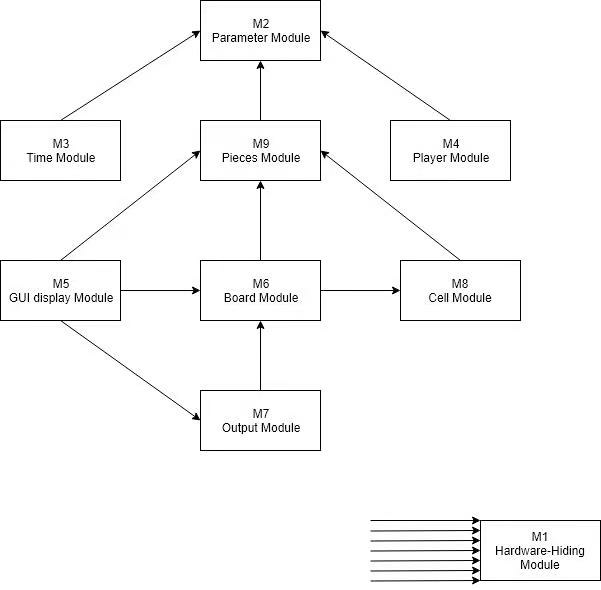
\includegraphics[width=0.7\textwidth]{UsesHierarchy.png}
\textcolor{red}{\caption{Use hierarchy among modules}}
\label{FigUH}
\end{figure}

%\section*{References}

\bibliographystyle {plainnat}
\bibliography {MG}

\end{document}